\chapter{Work Packages}
\label{ch:WP}

\section{Translator}
\paragraph{}
In a hierarchical architecture involving different MANOs, there is a need of conversion of network descriptors to schemas of respective MANO. Service Descriptor Translator (SDT) serves the purpose of translating network descriptors, namely NSDs and VNFDs from schema of SONATA Pishahang to that of OSM and vice versa.
\paragraph{}
In a scenario, where a parent MANO, say Pishahang decides to deploy one of the network services in its lower hierarchy MANO, say OSM, the NSD and VNFD(s) need to be converted to the descriptor schema of OSM. In such an event, the Scramble plugin calls the translator service and sends the descriptors to the SDT, where the translation of the descriptors takes place and the translated descriptors are sent to Adaptor utility for deployment in appropriate MANO. Figure \ref{fig:service-descriptor-translator} gives a high level view of Translator.
\paragraph{}
Scramble plug-in installed within the parent MANO forwards the network descriptors with service request to Scramble Main-Engine. Main-Engine checks the service request and sends the network descriptors to Translator along with the information of destination schema. On receiving the network descriptors, SDT translates the same to requested schema and calls the validator function to validate the translated network descriptors. Once validation is complete, the translated descriptors will be sent to Adaptor for deployment. 




\begin{figure}
	\centering
	\includegraphics[width=1\linewidth]{"figures/Service Descriptor Translator"}
	\caption{}
	\label{fig:service-descriptor-translator}
\end{figure}

\subsection{Architecture \& Work flow}
\subsection{usage}

+ code snippets and explanations

\subsection{challenges}
\subsection{Future scope of this work package}

\section{Splitter}
Communication between MANO frameworks and Scramble happens through plug-ins. Plug-ins will have some random logic to generate a multiple set of Network Functions into which a Network Service needs to be divided. The multiple set of NFs is then forwarded to Gateway micro-service along with the NS file which just receives the request and forward it to the Main-Engine. The Main Engine acts as an interface to all three utilities including Splitter. Main engine is responsible for interoperability and communication between all utilities. All three utilities are containerized using docker for easy distribution and scaling. Once the Splitter receives the request for splitting along with the parameters it splits the NSD into sub NSDs.
\subsection{Architecture \& Work flow}
Before actual splitting of NSD, Splitter first validates if the the multiple set it received is valid or not. Following things are validated by the splitter.
\begin{itemize}
	\item The total number of NFs mentioned in all the set matches the number of NFs defined in the NSD.
	\item There are no invalid NFs in the sets received.
\end{itemize}

After validation the actual splitting starts. We have created classes for different sections of a NSD which encapsulate all the attributes and its values into a single unit which makes it very easy to process. Once the objects are set they are passed to different splitting functions based on there type. We have two different processing units for OSM and SONATA. Following are some functions responsible for splitting the NSD.

\begin{itemize}
	\item \textbf{Set General information: }This function copies all the general information from the main NSD to the sub NSDs. Information includes Vendor, author, Version, Descripton etc.
	\item \textbf{Split Network Functions: }This function splits the Network functions from NSD to sub sets according to the request parameter received. 
	\item \textbf{Split Virtual Links: }When a NSD is splitted into different parts, its topology changes. Change in topology results in changing of Virtual Links. For example if A, B and C are three Nfs and we are splitting them in such a way so that A and B remain in one NSD and C in separate NSD. A virtual link between B and C now does not make sense. So this link should be broken down and B’s output should be connected to the external end point which was connected to C’s input earlier. This function splits these kind of Virtual Links.
	\item \textbf{Split Forwarding Graph: }As explained in the above section, once the topology changes, the respective Forwarding graph also changes. Split forwarding graph pulls out the set of connection points and newly created virtual links and sets them in the sub NSDs.
\end{itemize} 

Once the Splitting is done, create file is responsible for creating YAML files depending on the number of sub NSDs created. These files are saved in the file system which can be downloaded or moved forward to the adopter for deployment purpose. Following figure \ref{fig:splitter} graphically represents the splitting architecture.

\begin{figure} [h]
	\centering
	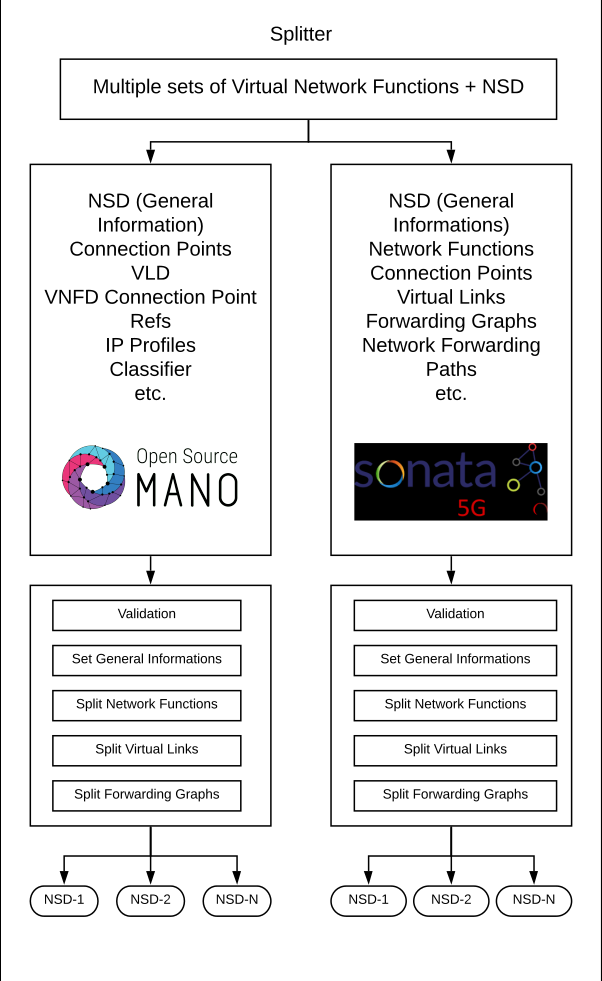
\includegraphics[width=0.5\linewidth]{figures/splitter}
	\caption{Scramble Architecture}
	\label{fig:splitter}
\end{figure}
\subsection{usage}

+ code snippets and explanations

\subsection{challenges}
\subsection{Future scope of this work package}

\section{Adaptor}
Python MANO Wrappers (PMW) is a uniform python wrapper library for various implementations of NFV Management and Network Orchestration (MANO) REST APIs. PMW is intended to ease the communication between python and MANO by providing a unified, convenient and standards oriented access to MANO API.

To achieve this, PMW follows the conventions from the ETSI GS NFV-SOL 005 (SOL005) RESTful protocols specification. This makes it easy to follow and the developers can use similar processes when communicating with a variety of MANO implementations.\\

PMW is easy to use and well documented. Code usage examples are available along with the detailed documentation at the following link \url{https://python-mano-wrappers.readthedocs.io/en/adaptor/}. \\

PMW in scramble helps in inter communication of different instances of MANO, thereby creating opportunity for more advanced feature set, for example, hierarchical scaling. Operations such as on-boarding of NSD and VNFD, instantiation and termination of NS can be performed with ease.

\subsection{Architecture \& Work flow}
Standards based approach is a fundamental design principle behind PMW's design. A Common interface template is defined in compliance with SOL005 which contains the blueprint for all the methods mentioned in the standards. These methods are divided into different sections as per SOL005 into the following:

\begin{itemize}
	\item \textbf{auth: }Authorization API
	\item \textbf{nsd: }NSD Management API
	\item \textbf{nsfm: }NS Fault Management API
	\item \textbf{nslcm: }Lifecycle Management API
	\item \textbf{nspm: }NS Performance Management API
	\item \textbf{vnfpkgm: }VNF Package Management API
\end{itemize} 

In the figure \ref{fig:wrapperarch}, different sections of PMW are visualized. As part of the scramble project, support for Open Source MANO (OSM) and Sonata is developed. This is represented by the dotted lines to OSM and Sonata modules. These modules are based on the common interface and implement the methods it has defined.

\subsection{usage}

+ code snippets and explanations


\subsection{Installation}
\subsection{challenges}
\subsection{Future scope of this work package}

